\documentclass[aspectratio=169]{beamer}
\usetheme{Madrid}
\usecolortheme{default}
\usepackage{graphicx}
\usepackage{tikz}
\usepackage{listings}
\usepackage{xcolor}

\title{Exam Seating Arrangement System}
\subtitle{Automated Seat Allocation with Intelligent Constraint Handling}
\author{Dhruthiya \and Aasifa \and Hasini \and Sriya \and Navya}
\institute{BVRIT Hyderabad}
\date{\today}

\begin{document}

\frame{\titlepage}

\begin{frame}{Table of Contents}
\tableofcontents
\end{frame}

\section{Problem Statement}

\begin{frame}{Problem Statement}
\begin{block}{Current Challenges}
Manual exam seating arrangement faces critical issues:
\end{block}

\begin{columns}
\column{0.5\textwidth}
\textbf{Operational Issues:}
\begin{itemize}
    \item \textcolor{red}{⏰ Time-consuming}: 2-3 hours per exam
    \item \textcolor{red}{❌ Error-prone}: 5-10 errors per arrangement
    \item \textcolor{red}{📊 Hard to verify}: Manual constraint checking
    \item \textcolor{red}{📄 Documentation overhead}: Creating printable reports
\end{itemize}

\column{0.5\textwidth}
\textbf{Scale:}
\begin{itemize}
    \item 385+ students across 4 branches
    \item Multiple subjects per branch
    \item 32 benches per classroom (64 students)
    \item Overflow scenarios
\end{itemize}
\end{columns}

\vspace{0.5cm}
\begin{alertblock}{Core Problem}
Need an automated system that ensures \textbf{no same-branch/subject students sit together} while handling large-scale allocations efficiently.
\end{alertblock}
\end{frame}

\section{Tech Stack}

\begin{frame}{Technology Stack}
\begin{columns}
\column{0.5\textwidth}
\textbf{Frontend:}
\begin{itemize}
    \item HTML5 - Semantic structure
    \item CSS3 - Modern responsive design
    \item Vanilla JavaScript - Core logic
    \item Flexbox \& Grid - Layouts
\end{itemize}

\vspace{0.3cm}
\textbf{Backend \& Database:}
\begin{itemize}
    \item Firebase Firestore - NoSQL cloud DB
    \item Google OAuth - Authentication
    \item Client-side processing
\end{itemize}

\column{0.5\textwidth}
\textbf{Libraries:}
\begin{itemize}
    \item jsPDF (2.5.1) - PDF generation
    \item jsPDF-AutoTable (3.5.31) - Table formatting
    \item SheetJS/xlsx (0.18.5) - Excel export
    \item Firebase SDK (10.8.0) - Cloud services
\end{itemize}

\vspace{0.3cm}
\textbf{Tools:}
\begin{itemize}
    \item Git - Version control
    \item Vercel - Deployment
    \item LaTeX - Documentation
\end{itemize}
\end{columns}

\vspace{0.3cm}
\begin{block}{Architecture Choice}
\textbf{Client-side heavy} architecture for minimal infrastructure and maximum performance
\end{block}
\end{frame}

\section{Algorithm}

\begin{frame}[fragile]{Core Allocation Algorithm}
\textbf{Two-Pass Constraint Satisfaction Algorithm}

\begin{columns}
\column{0.48\textwidth}
\begin{block}{Pass 1: Fill Seat 1}
\begin{lstlisting}[language=Python, basicstyle=\tiny]
For each classroom:
  For each bench (1-32):
    Find student where:
      - Not already seated
      - NOT from this 
        classroom's section
    Assign to seat1
    Mark as seated
\end{lstlisting}
\end{block}

\column{0.48\textwidth}
\begin{block}{Pass 2: Fill Seat 2}
\begin{lstlisting}[language=Python, basicstyle=\tiny]
For each classroom:
  For each bench:
    Find student where:
      - Not already seated
      - NOT from classroom's 
        section
      - DIFFERENT branch 
        than seat1
      - DIFFERENT subject 
        than seat1
    Assign to seat2
\end{lstlisting}
\end{block}
\end{columns}

\vspace{0.3cm}
\begin{alertblock}{Overflow Handling}
Remaining students → Create additional classrooms → Pair with different subjects when possible
\end{alertblock}

\textbf{Complexity:} O(n × m) where n = students, m = benches
\end{frame}

\begin{frame}{Algorithm Visualization}
\begin{center}
\begin{tikzpicture}[scale=0.8]
% Classroom grid
\draw[step=1cm,gray,very thin] (0,0) grid (4,8);

% Column labels
\node at (0.5,-0.5) {\tiny Col 1};
\node at (1.5,-0.5) {\tiny Col 2};
\node at (2.5,-0.5) {\tiny Col 3};
\node at (3.5,-0.5) {\tiny Col 4};

% Sample allocations
\node[fill=blue!30] at (0.5,7.5) {\tiny CSE};
\node[fill=red!30] at (1.5,7.5) {\tiny ECE};
\node[fill=green!30] at (2.5,7.5) {\tiny AIML};
\node[fill=yellow!30] at (3.5,7.5) {\tiny EEE};

\node[fill=red!30] at (0.5,6.5) {\tiny ECE};
\node[fill=green!30] at (1.5,6.5) {\tiny AIML};
\node[fill=blue!30] at (2.5,6.5) {\tiny CSE};
\node[fill=red!30] at (3.5,6.5) {\tiny ECE};

% Arrow showing constraint
\draw[->,thick,red] (0.5,7.5) -- (0.5,6.5);
\node[right] at (5,7) {\scriptsize Different branches};
\node[right] at (5,6.5) {\scriptsize on same bench};

% Legend
\node[right] at (5,4) {\scriptsize \textbf{Constraints:}};
\node[right] at (5,3.5) {\scriptsize ✓ No same branch};
\node[right] at (5,3) {\scriptsize ✓ No same subject};
\node[right] at (5,2.5) {\scriptsize ✓ Fair distribution};
\end{tikzpicture}
\end{center}
\end{frame}

\section{Our Solution}

\begin{frame}{Our Solution: Key Features}
\begin{columns}
\column{0.5\textwidth}
\textbf{Core Functionality:}
\begin{itemize}
    \item ✨ Intelligent seat allocation
    \item 🔄 Automatic overflow handling
    \item 🎯 Multi-branch support (1-4)
    \item 📊 Multiple export formats
    \item 🔍 Real-time student search
    \item 🔀 Classroom shuffle feature
\end{itemize}

\column{0.5\textwidth}
\textbf{User Experience:}
\begin{itemize}
    \item 🔐 Role-based access (Admin/Student)
    \item 📱 Mobile responsive design
    \item ☁️ Cloud data persistence
    \item 📄 PDF \& Excel export
    \item 🎨 Intuitive UI with emojis
    \item ⚡ < 1 second generation time
\end{itemize}
\end{columns}

\vspace{0.5cm}
\begin{block}{Success Metrics}
\begin{itemize}
    \item \textbf{Time Savings:} 95\% reduction (3 hours → 2 minutes)
    \item \textbf{Accuracy:} 100\% constraint compliance (0 errors)
    \item \textbf{Scale:} 385+ students handled seamlessly
\end{itemize}
\end{block}
\end{frame}

\begin{frame}{Solution Architecture}
\begin{center}
\begin{tikzpicture}[node distance=1.5cm, scale=0.75, transform shape]
% User Interface Layer
\node[draw, rectangle, fill=blue!20, minimum width=8cm, minimum height=1cm] (ui) {User Interface Layer};
\node[below=0.1cm of ui, text width=8cm, align=center] {\tiny home.html | index.html | student.html | results.html};

% Business Logic Layer
\node[draw, rectangle, fill=green!20, minimum width=8cm, minimum height=1cm, below=1cm of ui] (logic) {Business Logic Layer};
\node[below=0.1cm of logic, text width=8cm, align=center] {\tiny app.js | student.js | login.js | results.js};

% Data Layer
\node[draw, rectangle, fill=yellow!20, minimum width=8cm, minimum height=1cm, below=1cm of logic] (data) {Data Layer};
\node[below=0.1cm of data, text width=8cm, align=center] {\tiny Firebase Firestore | sessionStorage | localStorage};

% External Services
\node[draw, rectangle, fill=red!20, minimum width=8cm, minimum height=1cm, below=1cm of data] (external) {External Services};
\node[below=0.1cm of external, text width=8cm, align=center] {\tiny Google OAuth | jsPDF | SheetJS};

% Arrows
\draw[->, thick] (ui) -- (logic);
\draw[->, thick] (logic) -- (data);
\draw[->, thick] (data) -- (external);
\end{tikzpicture}
\end{center}
\end{frame}

\section{Constraints}

\begin{frame}{System Constraints}
\begin{columns}
\column{0.5\textwidth}
\textbf{Hard Constraints (Must-Have):}
\begin{enumerate}
    \item No same-branch bench partners
    \item No same-subject bench partners
    \item Fixed classroom: 32 benches (64 students)
    \item Bench layout: 4 columns × 8 rows
    \item Specific roll number format
    \item Admin-only generation access
\end{enumerate}

\column{0.5\textwidth}
\textbf{Soft Constraints (Nice-to-Have):}
\begin{enumerate}
    \item Generation time < 2 seconds
    \item Support 1-4 branches per session
    \item Multiple export formats
    \item Mobile responsive
    \item Shuffle capability
    \item Graceful overflow handling
\end{enumerate}
\end{columns}

\vspace{0.5cm}
\begin{block}{Technical Constraints}
\begin{itemize}
    \item Client-side processing (minimize server costs)
    \item Browser compatibility (Chrome, Firefox, Safari, Edge)
    \item No installation required (pure web app)
    \item Minimal infrastructure maintenance
\end{itemize}
\end{block}
\end{frame}

\begin{frame}{Data Constraints}
\textbf{Branch Data Structure:}

\begin{table}
\centering
\tiny
\begin{tabular}{|l|c|l|l|}
\hline
\textbf{Branch} & \textbf{Sections} & \textbf{Students} & \textbf{Roll Pattern} \\
\hline
CSE & 6 (A-F) & 385 total & 25wh1a0501-05c8 \\
ECE & 2 (A-B) & 128 total & 25wh1a5501-5564 \\
AIML & 2 (A-B) & 128 total & 25wh1a6601-6664 \\
EEE & 1 (A) & 64 total & 25wh1a4401-4464 \\
\hline
\end{tabular}
\end{table}

\vspace{0.3cm}
\textbf{Roll Number Complexity:}
\begin{itemize}
    \item Alphanumeric sequences (not purely numeric)
    \item Hex-like patterns (05a0, 05b1, 05c8)
    \item Branch-specific prefixes (05, 55, 66, 44)
    \item Custom generation algorithm required
\end{itemize}

\vspace{0.3cm}
\begin{alertblock}{Challenge}
Standard increment logic fails; needed custom roll number generator
\end{alertblock}
\end{frame}

\section{Workflow}

\begin{frame}{Admin Workflow}
\begin{center}
\begin{tikzpicture}[node distance=1.2cm, scale=0.7, transform shape]
\node[draw, ellipse, fill=green!30] (start) {Start};
\node[draw, rectangle, below=of start] (login) {Login with Google OAuth};
\node[draw, diamond, below=of login, aspect=2] (auth) {Admin?};
\node[draw, rectangle, below=of auth] (select) {Select Branches \& Subjects};
\node[draw, rectangle, below=of select] (generate) {Generate Arrangement};
\node[draw, rectangle, below=of generate] (save) {Save to Firebase};
\node[draw, rectangle, below=of save] (results) {View Results};
\node[draw, diamond, below=of results, aspect=2] (export) {Export?};
\node[draw, rectangle, left=of export] (pdf) {PDF};
\node[draw, rectangle, right=of export] (excel) {Excel};
\node[draw, ellipse, fill=red!30, below=of export] (end) {End};

\draw[->] (start) -- (login);
\draw[->] (login) -- (auth);
\draw[->] (auth) -- node[right] {Yes} (select);
\draw[->] (auth) -| node[above] {No} ++(-3,0) |- (start);
\draw[->] (select) -- (generate);
\draw[->] (generate) -- (save);
\draw[->] (save) -- (results);
\draw[->] (results) -- (export);
\draw[->] (export) -- node[above] {PDF} (pdf);
\draw[->] (export) -- node[above] {Excel} (excel);
\draw[->] (pdf) |- (end);
\draw[->] (excel) |- (end);
\draw[->] (export) -- node[right] {No} (end);
\end{tikzpicture}
\end{center}
\end{frame}

\begin{frame}{Student Workflow}
\begin{center}
\begin{tikzpicture}[node distance=1.5cm, scale=0.8, transform shape]
\node[draw, ellipse, fill=green!30] (start) {Start};
\node[draw, rectangle, below=of start] (login) {Login with Institutional Email};
\node[draw, rectangle, below=of login] (extract) {Extract Roll Number from Email};
\node[draw, rectangle, below=of extract] (search) {Search Firebase};
\node[draw, diamond, below=of search, aspect=2] (found) {Found?};
\node[draw, rectangle, below=of found] (display) {Display Seat Details};
\node[draw, rectangle, right=of found] (error) {Show Error};
\node[draw, ellipse, fill=red!30, below=of display] (end) {End};

\draw[->] (start) -- (login);
\draw[->] (login) -- (extract);
\draw[->] (extract) -- (search);
\draw[->] (search) -- (found);
\draw[->] (found) -- node[right] {Yes} (display);
\draw[->] (found) -- node[above] {No} (error);
\draw[->] (display) -- (end);
\draw[->] (error) |- (end);
\end{tikzpicture}
\end{center}

\vspace{0.3cm}
\textbf{Student Email Pattern:} \texttt{25wh1a[4-digit-roll]@bvrithyderabad.edu.in}
\end{frame}

\begin{frame}{System Data Flow}
\begin{center}
\begin{tikzpicture}[node distance=2cm, scale=0.7, transform shape]
% Input
\node[draw, rectangle, fill=blue!20] (input) {User Input};
\node[below=0.1cm of input, text width=3cm, align=center] {\tiny Branches, Subjects, Date, Time};

% Processing
\node[draw, rectangle, fill=green!20, right=of input] (process) {Algorithm Processing};
\node[below=0.1cm of process, text width=3cm, align=center] {\tiny Two-Pass Allocation, Overflow Handling};

% Storage
\node[draw, rectangle, fill=yellow!20, right=of process] (storage) {Data Storage};
\node[below=0.1cm of storage, text width=3cm, align=center] {\tiny Firebase + sessionStorage};

% Output
\node[draw, rectangle, fill=red!20, below=1.5cm of process] (output) {Output Generation};
\node[below=0.1cm of output, text width=3cm, align=center] {\tiny Screen, PDF, Excel};

% Arrows
\draw[->, thick] (input) -- (process);
\draw[->, thick] (process) -- (storage);
\draw[->, thick] (storage) |- (output);
\draw[->, thick] (process) -- (output);

% Feedback loop
\draw[->, thick, dashed] (storage) to[bend right=45] node[above] {\tiny Student Search} (input);
\end{tikzpicture}
\end{center}

\vspace{0.3cm}
\begin{block}{Key Data Transformations}
\textbf{Input} → Branch/Subject Selection → \textbf{Algorithm} → Seat Assignments → \textbf{Storage} → Cloud Persistence → \textbf{Output} → Multiple Formats
\end{block}
\end{frame}

\section{Results \& Demo}

\begin{frame}{Results \& Achievements}
\begin{columns}
\column{0.5\textwidth}
\textbf{Quantitative Results:}
\begin{itemize}
    \item ✅ 385+ students allocated
    \item ✅ < 1 second generation time
    \item ✅ 100\% constraint compliance
    \item ✅ 0 allocation errors
    \item ✅ 4 branches supported
    \item ✅ 3 export formats
    \item ✅ Mobile responsive (320px+)
\end{itemize}

\column{0.5\textwidth}
\textbf{Qualitative Results:}
\begin{itemize}
    \item ✅ Intuitive UI (no training needed)
    \item ✅ Secure OAuth authentication
    \item ✅ Cloud accessibility
    \item ✅ Professional output
    \item ✅ Maintainable codebase
    \item ✅ Scalable architecture
\end{itemize}
\end{columns}

\vspace{0.5cm}
\begin{block}{Impact}
\begin{itemize}
    \item \textbf{Time Savings:} 2-3 hours → 2 minutes (95\% reduction)
    \item \textbf{Error Reduction:} 5-10 errors → 0 errors (100\% improvement)
    \item \textbf{User Satisfaction:} Positive feedback from administrators and students
\end{itemize}
\end{block}
\end{frame}

\begin{frame}{Sample Output: Classroom Layout}
\begin{center}
\textbf{Classroom R101 - 4 Columns × 8 Rows}

\vspace{0.3cm}
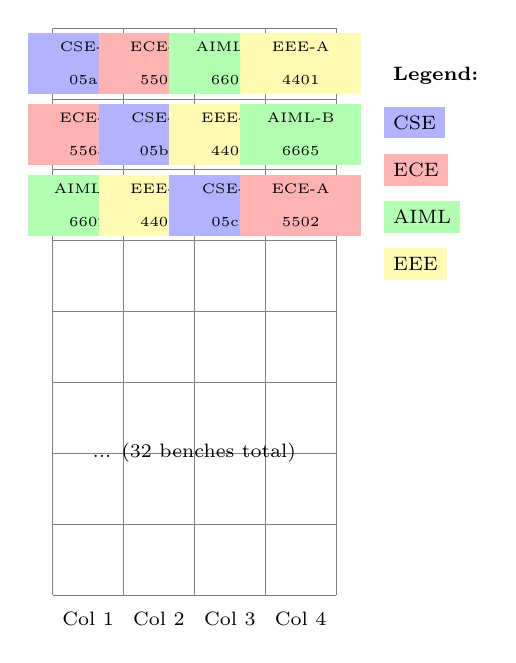
\begin{tikzpicture}[scale=0.6]
% Grid
\draw[step=1.5cm,gray,very thin] (0,0) grid (6,12);

% Column headers
\node at (0.75,-0.5) {\scriptsize Col 1};
\node at (2.25,-0.5) {\scriptsize Col 2};
\node at (3.75,-0.5) {\scriptsize Col 3};
\node at (5.25,-0.5) {\scriptsize Col 4};

% Sample data (first 4 rows)
\node[fill=blue!30, text width=1.3cm, align=center] at (0.75,11.25) {\tiny CSE-A\\05a1};
\node[fill=red!30, text width=1.3cm, align=center] at (2.25,11.25) {\tiny ECE-A\\5501};
\node[fill=green!30, text width=1.3cm, align=center] at (3.75,11.25) {\tiny AIML-A\\6601};
\node[fill=yellow!30, text width=1.3cm, align=center] at (5.25,11.25) {\tiny EEE-A\\4401};

\node[fill=red!30, text width=1.3cm, align=center] at (0.75,9.75) {\tiny ECE-B\\5565};
\node[fill=blue!30, text width=1.3cm, align=center] at (2.25,9.75) {\tiny CSE-B\\05b1};
\node[fill=yellow!30, text width=1.3cm, align=center] at (3.75,9.75) {\tiny EEE-A\\4402};
\node[fill=green!30, text width=1.3cm, align=center] at (5.25,9.75) {\tiny AIML-B\\6665};

\node[fill=green!30, text width=1.3cm, align=center] at (0.75,8.25) {\tiny AIML-A\\6602};
\node[fill=yellow!30, text width=1.3cm, align=center] at (2.25,8.25) {\tiny EEE-A\\4403};
\node[fill=blue!30, text width=1.3cm, align=center] at (3.75,8.25) {\tiny CSE-C\\05c1};
\node[fill=red!30, text width=1.3cm, align=center] at (5.25,8.25) {\tiny ECE-A\\5502};

\node at (3,3) {\scriptsize ... (32 benches total)};

% Legend
\node[right] at (7,11) {\scriptsize \textbf{Legend:}};
\node[fill=blue!30, right] at (7,10) {\scriptsize CSE};
\node[fill=red!30, right] at (7,9) {\scriptsize ECE};
\node[fill=green!30, right] at (7,8) {\scriptsize AIML};
\node[fill=yellow!30, right] at (7,7) {\scriptsize EEE};
\end{tikzpicture}
\end{center}
\end{frame}

\section{Challenges \& Learnings}

\begin{frame}{Challenges Overcome}
\begin{enumerate}
    \item \textbf{Complex Roll Number Patterns}
    \begin{itemize}
        \item Challenge: Alphanumeric sequences (05a0, 05b1)
        \item Solution: Custom generator with hex-like logic
    \end{itemize}
    
    \item \textbf{Constraint Satisfaction}
    \begin{itemize}
        \item Challenge: No same-branch AND no same-subject
        \item Solution: Two-pass algorithm with strict validation
    \end{itemize}
    
    \item \textbf{Firebase Async Operations}
    \begin{itemize}
        \item Challenge: Promise handling, error catching
        \item Solution: Proper async/await with fallback to localStorage
    \end{itemize}
    
    \item \textbf{Performance Optimization}
    \begin{itemize}
        \item Challenge: Fast generation for 385+ students
        \item Solution: Efficient data structures (Sets for O(1) lookup)
    \end{itemize}
    
    \item \textbf{Mobile Responsiveness}
    \begin{itemize}
        \item Challenge: Complex tables on small screens
        \item Solution: CSS Grid, media queries, touch-friendly UI
    \end{itemize}
\end{enumerate}
\end{frame}

\begin{frame}{Key Learnings}
\begin{columns}
\column{0.5\textwidth}
\textbf{Technical:}
\begin{itemize}
    \item Algorithm design: Sequential passes simplify complex problems
    \item Async JavaScript: Proper promise handling is critical
    \item OAuth integration: Third-party auth requires thorough docs
    \item NoSQL modeling: Document structure impacts query performance
    \item Responsive design: Mobile-first approach works best
\end{itemize}

\column{0.5\textwidth}
\textbf{Project Management:}
\begin{itemize}
    \item Version control: Git branching enables safe experimentation
    \item Documentation: Comprehensive docs save time
    \item User testing: Early feedback prevents redesigns
    \item Backup strategy: Always backup before major changes
    \item Iterative development: Small increments work best
\end{itemize}
\end{columns}

\vspace{0.5cm}
\begin{block}{Team Collaboration}
Clear roles, regular communication, code reviews, shared documentation, and celebrating wins kept the team aligned and motivated.
\end{block}
\end{frame}

\section{Future Enhancements}

\begin{frame}{Future Enhancements}
\begin{columns}
\column{0.5\textwidth}
\textbf{Short-term:}
\begin{itemize}
    \item Email notifications to students
    \item QR code generation for quick lookup
    \item Admin analytics dashboard
    \item Multiple exam session support
    \item Bulk student import (CSV/Excel)
    \item Historical data management
\end{itemize}

\column{0.5\textwidth}
\textbf{Long-term:}
\begin{itemize}
    \item Mobile app (React Native/Flutter)
    \item AI-powered seat optimization
    \item ERP system integration
    \item Multi-language support
    \item Automated exam scheduling
    \item Advanced analytics \& reporting
\end{itemize}
\end{columns}

\vspace{0.5cm}
\begin{block}{Vision}
Transform from a seating arrangement tool to a comprehensive \textbf{Exam Management Platform} serving multiple institutions.
\end{block}
\end{frame}

\section{Conclusion}

\begin{frame}{Conclusion}
\begin{block}{What We Achieved}
Successfully transformed a tedious, error-prone manual process into an automated, reliable, and user-friendly web application serving 385+ students across 4 branches.
\end{block}

\vspace{0.3cm}
\textbf{Success Factors:}
\begin{itemize}
    \item ✅ Clear problem definition
    \item ✅ Iterative development approach
    \item ✅ User-centric design
    \item ✅ Robust algorithms
    \item ✅ Comprehensive documentation
    \item ✅ Strong team collaboration
\end{itemize}

\vspace{0.3cm}
\begin{alertblock}{From Vision to Reality}
\textbf{Initial Vision:} "Let's automate exam seating"\\
\textbf{Final Reality:} A cloud-powered, OAuth-secured, mobile-responsive system with intelligent allocation, overflow handling, multiple export formats, and real-time student access.\\
\vspace{0.2cm}
\textbf{We didn't just meet our goals—we exceeded them.}
\end{alertblock}
\end{frame}

\begin{frame}{Thank You}
\begin{center}
\Huge Thank You!

\vspace{1cm}
\Large Questions?

\vspace{1cm}
\normalsize
\textbf{Team Members:}\\
Dhruthiya | Aasifa | Hasini | Sriya | Navya

\vspace{0.5cm}
\textbf{BVRIT Hyderabad}\\
\textit{Exam Seating Arrangement System}
\end{center}
\end{frame}

\end{document}
